% Options for packages loaded elsewhere
\PassOptionsToPackage{unicode}{hyperref}
\PassOptionsToPackage{hyphens}{url}
\PassOptionsToPackage{dvipsnames,svgnames,x11names}{xcolor}
%
\documentclass[
  a4paper,
]{scrreport}

\usepackage{amsmath,amssymb}
\usepackage{iftex}
\ifPDFTeX
  \usepackage[T1]{fontenc}
  \usepackage[utf8]{inputenc}
  \usepackage{textcomp} % provide euro and other symbols
\else % if luatex or xetex
  \usepackage{unicode-math}
  \defaultfontfeatures{Scale=MatchLowercase}
  \defaultfontfeatures[\rmfamily]{Ligatures=TeX,Scale=1}
\fi
\usepackage{lmodern}
\ifPDFTeX\else  
    % xetex/luatex font selection
\fi
% Use upquote if available, for straight quotes in verbatim environments
\IfFileExists{upquote.sty}{\usepackage{upquote}}{}
\IfFileExists{microtype.sty}{% use microtype if available
  \usepackage[]{microtype}
  \UseMicrotypeSet[protrusion]{basicmath} % disable protrusion for tt fonts
}{}
\makeatletter
\@ifundefined{KOMAClassName}{% if non-KOMA class
  \IfFileExists{parskip.sty}{%
    \usepackage{parskip}
  }{% else
    \setlength{\parindent}{0pt}
    \setlength{\parskip}{6pt plus 2pt minus 1pt}}
}{% if KOMA class
  \KOMAoptions{parskip=half}}
\makeatother
\usepackage{xcolor}
\setlength{\emergencystretch}{3em} % prevent overfull lines
\setcounter{secnumdepth}{-\maxdimen} % remove section numbering
% Make \paragraph and \subparagraph free-standing
\ifx\paragraph\undefined\else
  \let\oldparagraph\paragraph
  \renewcommand{\paragraph}[1]{\oldparagraph{#1}\mbox{}}
\fi
\ifx\subparagraph\undefined\else
  \let\oldsubparagraph\subparagraph
  \renewcommand{\subparagraph}[1]{\oldsubparagraph{#1}\mbox{}}
\fi

\usepackage{color}
\usepackage{fancyvrb}
\newcommand{\VerbBar}{|}
\newcommand{\VERB}{\Verb[commandchars=\\\{\}]}
\DefineVerbatimEnvironment{Highlighting}{Verbatim}{commandchars=\\\{\}}
% Add ',fontsize=\small' for more characters per line
\usepackage{framed}
\definecolor{shadecolor}{RGB}{241,243,245}
\newenvironment{Shaded}{\begin{snugshade}}{\end{snugshade}}
\newcommand{\AlertTok}[1]{\textcolor[rgb]{0.68,0.00,0.00}{#1}}
\newcommand{\AnnotationTok}[1]{\textcolor[rgb]{0.37,0.37,0.37}{#1}}
\newcommand{\AttributeTok}[1]{\textcolor[rgb]{0.40,0.45,0.13}{#1}}
\newcommand{\BaseNTok}[1]{\textcolor[rgb]{0.68,0.00,0.00}{#1}}
\newcommand{\BuiltInTok}[1]{\textcolor[rgb]{0.00,0.23,0.31}{#1}}
\newcommand{\CharTok}[1]{\textcolor[rgb]{0.13,0.47,0.30}{#1}}
\newcommand{\CommentTok}[1]{\textcolor[rgb]{0.37,0.37,0.37}{#1}}
\newcommand{\CommentVarTok}[1]{\textcolor[rgb]{0.37,0.37,0.37}{\textit{#1}}}
\newcommand{\ConstantTok}[1]{\textcolor[rgb]{0.56,0.35,0.01}{#1}}
\newcommand{\ControlFlowTok}[1]{\textcolor[rgb]{0.00,0.23,0.31}{#1}}
\newcommand{\DataTypeTok}[1]{\textcolor[rgb]{0.68,0.00,0.00}{#1}}
\newcommand{\DecValTok}[1]{\textcolor[rgb]{0.68,0.00,0.00}{#1}}
\newcommand{\DocumentationTok}[1]{\textcolor[rgb]{0.37,0.37,0.37}{\textit{#1}}}
\newcommand{\ErrorTok}[1]{\textcolor[rgb]{0.68,0.00,0.00}{#1}}
\newcommand{\ExtensionTok}[1]{\textcolor[rgb]{0.00,0.23,0.31}{#1}}
\newcommand{\FloatTok}[1]{\textcolor[rgb]{0.68,0.00,0.00}{#1}}
\newcommand{\FunctionTok}[1]{\textcolor[rgb]{0.28,0.35,0.67}{#1}}
\newcommand{\ImportTok}[1]{\textcolor[rgb]{0.00,0.46,0.62}{#1}}
\newcommand{\InformationTok}[1]{\textcolor[rgb]{0.37,0.37,0.37}{#1}}
\newcommand{\KeywordTok}[1]{\textcolor[rgb]{0.00,0.23,0.31}{#1}}
\newcommand{\NormalTok}[1]{\textcolor[rgb]{0.00,0.23,0.31}{#1}}
\newcommand{\OperatorTok}[1]{\textcolor[rgb]{0.37,0.37,0.37}{#1}}
\newcommand{\OtherTok}[1]{\textcolor[rgb]{0.00,0.23,0.31}{#1}}
\newcommand{\PreprocessorTok}[1]{\textcolor[rgb]{0.68,0.00,0.00}{#1}}
\newcommand{\RegionMarkerTok}[1]{\textcolor[rgb]{0.00,0.23,0.31}{#1}}
\newcommand{\SpecialCharTok}[1]{\textcolor[rgb]{0.37,0.37,0.37}{#1}}
\newcommand{\SpecialStringTok}[1]{\textcolor[rgb]{0.13,0.47,0.30}{#1}}
\newcommand{\StringTok}[1]{\textcolor[rgb]{0.13,0.47,0.30}{#1}}
\newcommand{\VariableTok}[1]{\textcolor[rgb]{0.07,0.07,0.07}{#1}}
\newcommand{\VerbatimStringTok}[1]{\textcolor[rgb]{0.13,0.47,0.30}{#1}}
\newcommand{\WarningTok}[1]{\textcolor[rgb]{0.37,0.37,0.37}{\textit{#1}}}

\providecommand{\tightlist}{%
  \setlength{\itemsep}{0pt}\setlength{\parskip}{0pt}}\usepackage{longtable,booktabs,array}
\usepackage{calc} % for calculating minipage widths
% Correct order of tables after \paragraph or \subparagraph
\usepackage{etoolbox}
\makeatletter
\patchcmd\longtable{\par}{\if@noskipsec\mbox{}\fi\par}{}{}
\makeatother
% Allow footnotes in longtable head/foot
\IfFileExists{footnotehyper.sty}{\usepackage{footnotehyper}}{\usepackage{footnote}}
\makesavenoteenv{longtable}
\usepackage{graphicx}
\makeatletter
\def\maxwidth{\ifdim\Gin@nat@width>\linewidth\linewidth\else\Gin@nat@width\fi}
\def\maxheight{\ifdim\Gin@nat@height>\textheight\textheight\else\Gin@nat@height\fi}
\makeatother
% Scale images if necessary, so that they will not overflow the page
% margins by default, and it is still possible to overwrite the defaults
% using explicit options in \includegraphics[width, height, ...]{}
\setkeys{Gin}{width=\maxwidth,height=\maxheight,keepaspectratio}
% Set default figure placement to htbp
\makeatletter
\def\fps@figure{htbp}
\makeatother

%\newfontfamily\Ubuntu[Mapping=tex-text]{Ubuntu}
\usepackage{pgfplots}
\usetikzlibrary{arrows.meta,arrows}
\usetikzlibrary{angles,quotes}
\pgfplotsset{grid style={dashed,mygray}}
% Colors
\definecolor{myblue}{rgb}{0.067,0.529,0.871}
\definecolor{mypurple}{rgb}{0.859,0.071,0.525}
\definecolor{myred}{rgb}{1.0, 0.13, 0.32}
\definecolor{mygreen}{rgb}{0.01, 0.75, 0.24}
\definecolor{myblack}{gray}{0.1}
\definecolor{mygray}{gray}{0.8}
\newcommand{\NN}{\mathbb{N}}
\newcommand{\ZZ}{\mathbb{Z}}
\newcommand{\QQ}{\mathbb{Q}}
\newcommand{\RR}{\mathbb{R}}
\newcommand{\CC}{\mathbb{C}}
\DeclareMathOperator{\Int}{Int}
\DeclareMathOperator{\Ext}{Ext}
\DeclareMathOperator{\Fr}{Fr}
\DeclareMathOperator{\Adh}{Adh}
\DeclareMathOperator{\Ac}{Ac}
\DeclareMathOperator{\sen}{sen}
\makeatletter
\@ifpackageloaded{caption}{}{\usepackage{caption}}
\AtBeginDocument{%
\ifdefined\contentsname
  \renewcommand*\contentsname{Indice de contenidos}
\else
  \newcommand\contentsname{Indice de contenidos}
\fi
\ifdefined\listfigurename
  \renewcommand*\listfigurename{Listado de Figuras}
\else
  \newcommand\listfigurename{Listado de Figuras}
\fi
\ifdefined\listtablename
  \renewcommand*\listtablename{Listado de Tablas}
\else
  \newcommand\listtablename{Listado de Tablas}
\fi
\ifdefined\figurename
  \renewcommand*\figurename{Figura}
\else
  \newcommand\figurename{Figura}
\fi
\ifdefined\tablename
  \renewcommand*\tablename{Tabla}
\else
  \newcommand\tablename{Tabla}
\fi
}
\@ifpackageloaded{float}{}{\usepackage{float}}
\floatstyle{ruled}
\@ifundefined{c@chapter}{\newfloat{codelisting}{h}{lop}}{\newfloat{codelisting}{h}{lop}[chapter]}
\floatname{codelisting}{Listado}
\newcommand*\listoflistings{\listof{codelisting}{Listado de Listados}}
\makeatother
\makeatletter
\makeatother
\makeatletter
\@ifpackageloaded{caption}{}{\usepackage{caption}}
\@ifpackageloaded{subcaption}{}{\usepackage{subcaption}}
\makeatother
\ifLuaTeX
\usepackage[bidi=basic]{babel}
\else
\usepackage[bidi=default]{babel}
\fi
\babelprovide[main,import]{spanish}
% get rid of language-specific shorthands (see #6817):
\let\LanguageShortHands\languageshorthands
\def\languageshorthands#1{}
\ifLuaTeX
  \usepackage{selnolig}  % disable illegal ligatures
\fi
\usepackage{bookmark}

\IfFileExists{xurl.sty}{\usepackage{xurl}}{} % add URL line breaks if available
\urlstyle{same} % disable monospaced font for URLs
\hypersetup{
  pdftitle={Sistema de cálculo simbólico},
  pdflang={es},
  colorlinks=true,
  linkcolor={blue},
  filecolor={Maroon},
  citecolor={Blue},
  urlcolor={Blue},
  pdfcreator={LaTeX via pandoc}}

\title{Sistema de cálculo simbólico}
\author{}
\date{}

\begin{document}
\begin{titlepage}

%\AddToShipoutPicture*{\put(0,0){\includegraphics[scale=0.8]{img/background2}}} % Imagen de fondo, requiere el paquete eso-pic.
\begin{center}
\vspace*{5cm}

\Huge
{\textbf{\textsf{Sistema de cálculo simbólico}}}

\vspace{0.5cm}
\LARGE
{\textbf{\textsf{}}}

\vspace{1.5cm}


\includegraphics[width=0.4\textwidth]{../img/logos/proyectos.png}
\end{center}

\vfill

\begin{flushleft}
\begin{tabular}{ll}

\includegraphics[width=0.1\textwidth]{../img/logos/aprendeconalf.png} & \parbox[b]{5cm}{\Large\textsf{}\\ \textsf{asalber@ceu.es} \\ \textsf{https://aprendeconalf.es}}
\end{tabular}
\end{flushleft}
\end{titlepage}
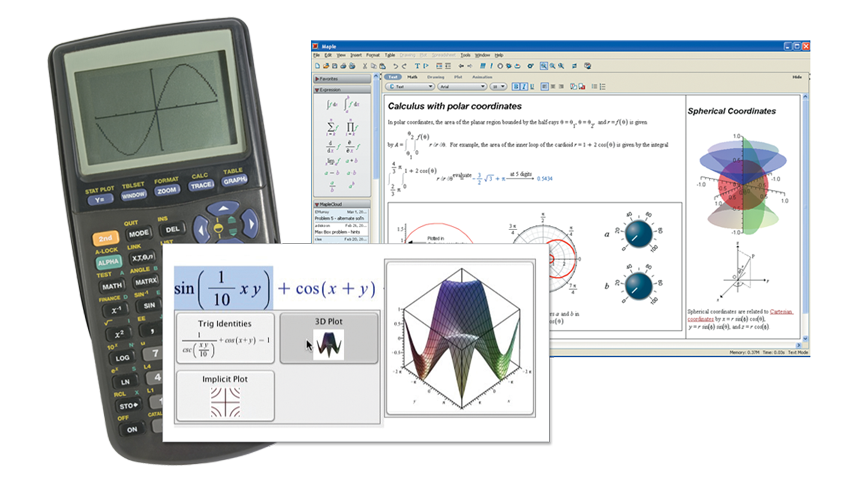
\includegraphics{../img/calculo-simbolico/cas.png}

\section{Introducción}\label{introducciuxf3n}

Un \emph{sistema de álgebra computacional} (CAS, del inglés computer
algebra system) es un programa de ordenador o calculadora avanzada que
facilita el cálculo simbólico. La principal diferencia entre un CAS y
una calculadora tradicional es la habilidad del primero para trabajar
con ecuaciones y fórmulas simbólicamente, en lugar de numéricamente.
Esto permite trabajar con expresiones simbólicas (no numéricas) y
realizar operaciones como la resolución de ecuaciones, el cálculo de
límites, el cálculo de derivadas o el cálculo de integrales.

\section{Objetivos}\label{objetivos}

El objetivo de este proyecto es desarrollar un sistema de álgebra
computacional para el cálculo simbólico que permita el cálculo de
derivadas, la resolución de ecuaciones y la simplificación de
expresiones.

\section{Descripción técnica}\label{descripciuxf3n-tuxe9cnica}

Para manejar expresiones simbólicas los sistemas de álgebra
computacional suelen representarlas mediante un árbol en el que las
operaciones forman los nodos y los argumentos son las ramas. Por
ejemplo, la expresión \(\dfrac{\cos(x+\pi)}{y^2}\) se representaría
mediante el árbol siguiente

\phantomsection\label{arbol-expresion}
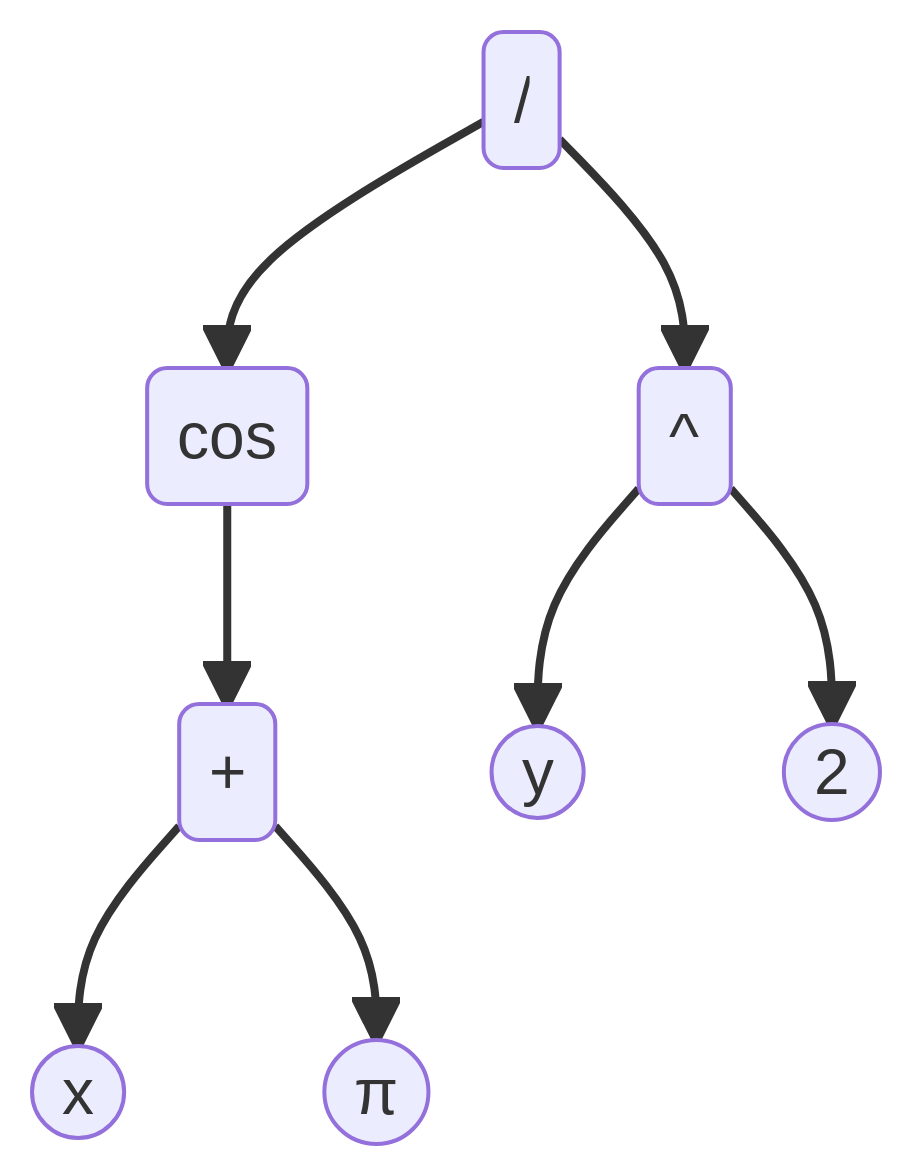
\includegraphics[width=2.37in,height=3.03in]{calculo-simbolico_files/figure-latex/mermaid-figure-1.png}

Árbol de la expresión \(\dfrac{\cos(x+\pi)}{y^2}\).

Julia dispone del tipo de datos \texttt{Expr} para las expresiones
simbólicas. Para definir un símbolo o una expresión simbólica se utiliza
el operador \texttt{:}.

\begin{Shaded}
\begin{Highlighting}[]
\NormalTok{ex }\OperatorTok{=} \OperatorTok{:}\NormalTok{(}\FunctionTok{sin}\NormalTok{(x}\OperatorTok{+}\ConstantTok{pi}\NormalTok{))}
\FunctionTok{typeof}\NormalTok{(ex)}
\end{Highlighting}
\end{Shaded}

\begin{verbatim}
Expr
\end{verbatim}

La principal diferencia entre una expresión normal y una expresión
simbólica es que esta última no se evalúa.

A su vez, el paquete de Julia \texttt{TermInterface} proporciona una
interfaz genérica para manipular expresiones simbólicas. Las tres
principales funciones de este paquete son

\begin{itemize}
\tightlist
\item
  \texttt{istree(ex)}: Devuelve \texttt{true} si \texttt{ex} es una
  expresión simbólica y \texttt{false} cuando se trata de un símbolo o
  un número.
\item
  \texttt{operation(ex)}: Devuelve el operador más externo de la
  expresión simbólica \texttt{ex}, es decir, el operador en la raíz del
  árbol correspondiente a la expresión.
\item
  \texttt{arguments(ex)}: Devuelve un vector con los argumentos sobre
  los que se aplica el operador máx externo de la expresión simbólica
  \texttt{ex}, es decir, un vector con las expresiones simbólicas
  correspondientes a cada una de las ramas que salen de la raíz del
  árbol correspondiente a la expresión. Dependiendo de la longitud de
  este vector se puede averiguar la aridad del operador, es decir, si es
  unario, binario o en general \(n\)-ario.
\end{itemize}

\begin{Shaded}
\begin{Highlighting}[]
\ImportTok{using} \BuiltInTok{TermInterface}
\FunctionTok{istree}\NormalTok{(}\OperatorTok{:}\NormalTok{(x}\OperatorTok{+}\FloatTok{2}\NormalTok{))}
\end{Highlighting}
\end{Shaded}

\begin{verbatim}
true
\end{verbatim}

\begin{Shaded}
\begin{Highlighting}[]
\FunctionTok{operation}\NormalTok{(}\OperatorTok{:}\NormalTok{(x}\OperatorTok{+}\FloatTok{2}\NormalTok{))}
\end{Highlighting}
\end{Shaded}

\begin{verbatim}
:+
\end{verbatim}

\begin{Shaded}
\begin{Highlighting}[]
\NormalTok{arg }\OperatorTok{=} \FunctionTok{arguments}\NormalTok{(}\OperatorTok{:}\NormalTok{(x}\OperatorTok{+}\FloatTok{2}\NormalTok{))}
\end{Highlighting}
\end{Shaded}

\begin{verbatim}
2-element Vector{Any}:
  :x
 2
\end{verbatim}

\begin{Shaded}
\begin{Highlighting}[]
\FunctionTok{isa}\NormalTok{(arg[}\FloatTok{1}\NormalTok{], }\DataTypeTok{Symbol}\NormalTok{)}
\end{Highlighting}
\end{Shaded}

\begin{verbatim}
true
\end{verbatim}

\begin{Shaded}
\begin{Highlighting}[]
\FunctionTok{isa}\NormalTok{(arg[}\FloatTok{2}\NormalTok{], }\DataTypeTok{Symbol}\NormalTok{)}
\end{Highlighting}
\end{Shaded}

\begin{verbatim}
false
\end{verbatim}

\section{Tareas}\label{tareas}

\begin{enumerate}
\def\labelenumi{\arabic{enumi}.}
\tightlist
\item
  Aprender a manejar expresiones simbólicas en Julia haciendo uso del
  paquete \texttt{TermInterface}.
\item
  Definir una función para dibujar el árbol correspondiente a una
  expresión simbólica.
\item
  Definir una función para calcular la derivada de una expresión
  simbólica.
\item
  Definir una función para resolver una ecuación simbólicamente.
\item
  Definir una función para simplificar una expresión simbólica.
\item
  Desarrollar una aplicación para una sistema de álgebra computacional
  que calcule derivadas, resuelva ecuaciones y simplifique expresiones
  simbólicas.
\end{enumerate}



\end{document}
